\documentclass{article}

\usepackage{subfigure}
\usepackage{amssymb, amsmath, amsfonts}
\usepackage{amsthm}
\usepackage{tikz}
\usetikzlibrary{external,matrix,arrows,fit,backgrounds,plotmarks,shapes.geometric}
\usepackage{pgfplots}

\newtheorem{proposition}{Proposition}
\newtheorem{theorem}{Theorem}
\newtheorem{definition}{Definition}
\newtheorem{lemma}{Lemma}
\newtheorem{conjecture}{Conjecture}
\newtheorem{corollary}{Corollary}
\newtheorem{remark}{Remark}
\newtheorem{assumption}{Assumption}

\newlength\figureheight
\newlength\figurewidth

\ifnum\pdfshellescape=1
\tikzexternalize[prefix=tikzpdf/]
\fi

\newcommand{\tikzdir}[1]{tikz/#1.tikz}
\newcommand{\why}{({\bf why?})}
\newcommand{\inputtikz}[1]{\tikzsetnextfilename{#1}\input{\tikzdir{#1}}}

\DeclareMathOperator*{\argmin}{arg\; min}     % argmin
\DeclareMathOperator*{\argmax}{arg\; max}     % argmax
\DeclareMathOperator*{\tr}{tr}     % trace
\DeclareMathOperator{\Cov}{Cov}
\DeclareMathOperator{\logdet}{log\;det}
\DeclareMathOperator{\der}{d}

\title{Lecture 2: State Estimation and Kalman Filter}

\author{Yilin Mo}

\begin{document} \maketitle
\section{Static State Estimation}
Let $x\in \mathbb R^n$ be the states and $y\in \mathbb R^m$ be the sensor measurements. The a-priori pdf of $x$ is $f(x)$ and the conditional pdf of $y$ given $x$ is $f(y|x)$. Hence,
\begin{displaymath}
  f(x|y) =  \frac{f(x,y)}{f(y)} = \frac{f(x)f(y|x)}{\int_{\mathbb R^n} f(x)f(y|x)\der x}.
\end{displaymath}
The minimum mean square error (MMSE) estimator is given by
\begin{displaymath}
  \hat x = \mathbb E(x|y) = \int_{R^n} xf(x|y)\der x. 
\end{displaymath}
\section{State Estimation of Hidden Markov Chain}
\begin{figure}[h]
  \begin{center}
    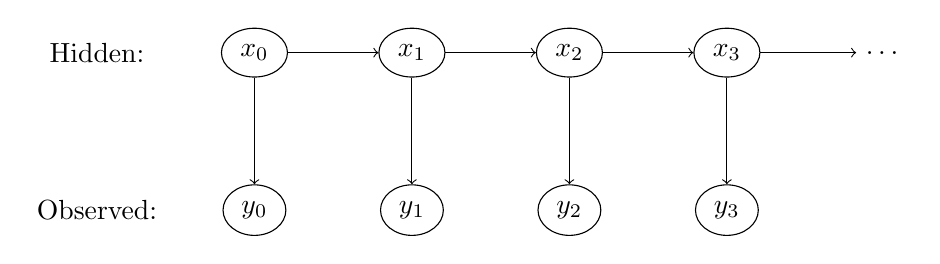
\begin{tikzpicture}
      \node at (0,2) {Hidden:};
      \node at (0,0) {Observed:};
      \node (x0) at (2,2) [ellipse,draw] {$x_0$};
      \node (y0) at (2,0) [ellipse,draw] {$y_0$};
      \draw [->](x0)--(y0);
      \node (x1) at (4,2) [ellipse,draw] {$x_1$};
      \node (y1) at (4,0) [ellipse,draw] {$y_1$};
      \draw [->](x1)--(y1);
      \draw [->](x0)--(x1);
      \node (x2) at (6,2) [ellipse,draw] {$x_2$};
      \node (y2) at (6,0) [ellipse,draw] {$y_2$};
      \draw [->](x2)--(y2);
      \draw [->](x1)--(x2);
      \node (x3) at (8,2) [ellipse,draw] {$x_3$};
      \node (y3) at (8,0) [ellipse,draw] {$y_3$};
      \draw [->](x3)--(y3);
      \draw [->](x2)--(x3);
      \node (future) at (10,2) {\dots};
      \draw [->](x3)--(future);
    \end{tikzpicture}
  \end{center}
  \caption{Hidden Markov Model}
\end{figure}
Markov Property: The joint pdf of $x_0,\dots,x_k$, $y_0,\dots,y_k$ satisfies:
\begin{displaymath}
  f(x_0,\dots,x_k,y_0,\dots,y_k) = f(x_0)\prod_{i=0}^{k-1}f(x_{i+1}|x_i)\prod_{i=0}^k f(y_i|x_i).
\end{displaymath}

To simplify notation, define $Y_k = (y_0,\dots,y_k)$ and $Y_{-1} = \emptyset$.

\subsection{Naive Estimator}
We can still use the conditional expectation to compute the MMSE estimator:
\begin{equation}
  \hat x_{k|k} = \mathbb E(x_k|Y_k).
  \label{eq:estimator1}
\end{equation}

{\bf Drawbacks:}

Estimator~\eqref{eq:estimator1} is not recursive. We need to keep the whole history of $Y_k$. 

\subsection{Bayes Filter}
Consider the conditional pdf $f(x_k|Y_k)$, by Bayes rule:
\begin{displaymath}
  f(x_k|Y_k) = \frac{f(x_k,y_k|Y_{k-1})}{f(y_k|Y_{k-1})} = \frac{f(y_k|x_k,Y_{k-1})f(x_k|Y_{k-1})}{f(y_k|Y_{k-1})} 
\end{displaymath}
\begin{enumerate}
  \item By Markov property:
    \begin{displaymath}
      f(y_k|x_k,Y_{k-1}) = f(y_k|x_k).
    \end{displaymath}
  \item By law of total probability and Markov property:
    \begin{align}
      f(x_k|Y_{k-1}) &= \int_{\mathbb R^n} f(x_k|x_{k-1}, Y_{k-1})f(x_{k-1}|Y_{k-1})\der x_{k-1}\nonumber\\
      &= \int_{\mathbb R^n} f(x_k|x_{k-1})f(x_{k-1}|Y_{k-1})\der x_{k-1}
      \label{eq:bayespredict}
    \end{align}
  \item By law of total probability and Markov property:
    \begin{align*}
      f(y_k|Y_{k-1}) & = \int_{\mathbb R^n} f(y_k|x_k,Y_{k-1}) f(x_k|Y_{k-1})\der x_k\\
      &= \int_{\mathbb R^n} f(y_k|x_k) f(x_k|Y_{k-1})\der x_k.
    \end{align*}
\end{enumerate}
As a result, the Bayes filter can be written in a recursive fashion as:
\begin{enumerate}
  \item {\bf Initialization:}
    \begin{displaymath}
      f(x_0|Y_{-1}) = f(x_0).
    \end{displaymath}
  \item {\bf Correction:}
    \begin{displaymath}
      f(x_k|Y_k) = \alpha f(y_k|x_k)f(x_k|Y_{k-1}),
    \end{displaymath}
    where
    \begin{displaymath}
      \alpha = \left(\int_{\mathbb R^n} f(y_k|x_k)f(x_k|Y_{k-1})\der x_k \right)^{-1}. 
    \end{displaymath}
    The MMSE estimation can be derived as
    \begin{displaymath}
      \hat x = \mathbb E(x_k|Y_k) = \int_{\mathbb R^n}x_kf(x_k|Y_k)\der x_k. 
    \end{displaymath}
  \item {\bf Prediction:}
    \begin{displaymath}
      f(x_{k+1}|Y_k) = \int_{\mathbb R^n} f(x_{k+1}|x_k)f(x_k|Y_k)\der x_k. 
    \end{displaymath}
\end{enumerate}

{\bf Drawbacks:}

we need to store the conditional pdf $f(x_k|Y_k)$ or $f(x_k|Y_{k-1})$.

{\bf Possible Solutions:}
\begin{itemize}
  \item Assuming that the conditional pdf is Gaussian. Hence, only need to track the mean and covariance (Extended Kalman Filter). 
  \item Approximating the conditional pdf by Monte Carlo sampling (Particle filter) 
\end{itemize}
\section{Estimation of Linear Gaussian System: Kalman Filter}
Consider the following linear Gaussian system:
\begin{align*}
  x_{k+1} &= A x_k + w_k,\\
y_k &= Cx_k + v_k.
\end{align*}
where the process noise $w_k$ is i.i.d. Gaussian noise with mean 0 and covariance $Q$. The measurement noise $v_k$ is i.i.d. Gaussian noise with mean 0 and covariance $R$ and the initial condition $x_0$ is Gaussian with mean 0 and covariance $\Sigma$. The random variables $\{x_0,w_0,\dots,w_k,v_0,\dots,v_k\}$ are jointly independent.

{\bf Observation:} $(x_0,\dots,x_k,y_0,\dots,y_k)$ are jointly Gaussian. Hence, the conditional pdf $f(x_k|Y_k)$ and $f(x_k|Y_{k-1})$ is also Gaussian. As a result, we only need to keep track of 
\begin{align*}
  \hat x_{k|k} &= \mathbb E(x_k|Y_k),\, \hat x_{k|k-1} = \mathbb E(x_k|Y_{k-1}),\\
  P_{k|k} &= \Cov(x_k|Y_k) = \mathbb E\left( (x_k - \hat x_{k|k})(x_k - \hat x_{k|k})^TY_k \right),\\
  P_{k|k-1} &=  \Cov(x_k|Y_{k-1}) = \mathbb E\left( (x_k - \hat x_{k|k-1})(x_k - \hat x_{k|k-1})^TY_{k-1} \right).
\end{align*}

\begin{enumerate}
  \item {\bf Initialization:}
    \begin{equation}
      \hat x_{0|-1} = 0,\,P_{0|-1} = \Sigma. 
      \label{eq:init}
    \end{equation}
  \item {\bf Prediction:} Take the conditional expectation on both sides of $x_{k+1} = Ax_k + w_k$, 
    \begin{displaymath}
      \mathbb E(x_{k+1}|Y_k) = A \mathbb E(x_k|Y_k) + \mathbb E(w_k | Y_k). 
    \end{displaymath}
    The second term on the RHS is $0$ \why. Hence
    \begin{equation}
      \hat x_{k+1|k} = A \hat x_{k|k}. 
      \label{eq:predict1}
    \end{equation}
    Therefore,
    \begin{displaymath}
      x_{k+1}-\hat x_{k+1|k} = A(x_k- \hat x_{k|k}) + w_k,
    \end{displaymath}
    which implies that
    \begin{align*}
     (x_{k+1}-\hat x_{k+1|k})(x_{k+1}-\hat x_{k+1|k})^T &= A(x_k- \hat x_{k|k})(x_k- \hat x_{k|k})^TA^T + w_kw_k^T  \\
     &+ A(x_k- \hat x_{k|k}) w_k^T + w_k(x_k- \hat x_{k|k})^TA^T.
    \end{align*}
    Take the conditional expectation on $Y_{k}$ on both sides. Notice that the conditional expectation of the last two terms on the RHS is 0 \why. Hence
    \begin{equation}
      P_{k+1|k} = AP_{k|k}A^T + Q. 
      \label{eq:predict2}
    \end{equation}
  \item {\bf Correction:} We need the following theorem:
    \begin{theorem}
      Assume that the joint pdf of $x,y$ satisfies
      \begin{displaymath}
	f\begin{pmatrix}x\\y\end{pmatrix}\sim\mathcal N\left(\begin{bmatrix}\mu_x\\ \mu_y\end{bmatrix},\begin{bmatrix}\Sigma_{xx}&\Sigma_{xy}\\ \Sigma_{xy}^T&\Sigma_{yy}\end{bmatrix}  \right),
      \end{displaymath}
      then the following equalities hold:
      \begin{align*}
	\mathbb E(x|y) &= \mu_x + \Sigma_{xy}\Sigma_{yy}^{-1} (y - \mu_y),\\
	\Cov(x|y) &= \Sigma_{xx} - \Sigma_{xy}\Sigma_{yy}^{-1}\Sigma_{xy}^T.
      \end{align*}
      \label{thm:conditionalgaussian}
    \end{theorem}

    By \eqref{eq:predict1} and \eqref{eq:predict2}, we already know that
    \begin{displaymath}
      \mathbb E(x_{k+1}|Y_k) = \hat x_{k+1|k},\, \Cov(x_{k+1}|Y_k) = P_{k+1|k}.
    \end{displaymath}

    Now take the conditional expectation on $Y_k$ on both sides of $y_{k+1} = Cx_{k+1} + v_{k+1}$, we get
    \begin{displaymath}
      \mathbb E(y_{k+1}|Y_k) = C \hat x_{k+1|k}. 
    \end{displaymath}
    Similar to the proof of \eqref{eq:predict2}, we have
    \begin{align*}
      \Cov(y_{k+1}|Y_k) &= CP_{k+1|k}C^T + R,\\ 
      \Cov(x_{k+1},y_{k+1}|Y_k)&=\mathbb E\left(  (x_{k+1}- \hat x_{k+1|k})(y_{k+1}- \mathbb E(y_{k+1}|Y_k) )^T|Y_k\right) = P_{k+1|k}C^T.
    \end{align*}
    Therefore, the joint pdf of $x_{k+1},y_{k+1}$ satisfies
    \begin{displaymath}
      f\left(   \left. \begin{bmatrix}x_{k+1}\\y_{k+1}\end{bmatrix} \right|Y_k \right)\sim\mathcal N\left( \begin{bmatrix}\hat x_{k+1|k}\\C\hat x_{k+1|k}\end{bmatrix}, \begin{bmatrix}P_{k+1|k}&P_{k+1|k}C^T\\CP_{k+1|k}&CP_{k+1|k}C^T + R\end{bmatrix} \right).
    \end{displaymath}
    Using Theorem~\ref{thm:conditionalgaussian}, we get the correction equations:
    \begin{align}
      \label{eq:correction1}
      \hat x_{k+1|k+1} &= \hat x_{k+1|k} + P_{k+1|k}C^T(CP_{k+1|k}C^T+R)^{-1}(y_{k+1} - C\hat x_{k+1|k}),\\
      \label{eq:correction2}
      P_{k+1|k+1} &= P_{k+1|k} - P_{k+1|k}C^T(CP_{k+1|k}C^T+R)^{-1}CP_{k+1|k}.
    \end{align}
\end{enumerate}
Equation \eqref{eq:init}, \eqref{eq:predict1}, \eqref{eq:predict2}, \eqref{eq:correction1} and \eqref{eq:correction2} are called Kalman filter.

{\bf Observations:}
\begin{itemize}
  \item $P_{k|k}, P_{k+1|k}$ do not depend on $Y_k$. Hence, they can be computed off-line.
  \item Define
    \begin{displaymath}
      K_k \triangleq P_{k|k-1}C^T(CP_{k|k-1}C^T+R)^{-1}. 
    \end{displaymath}
    Assume that $C$ is invertible.
    \begin{itemize}
      \item If $P_{k|k-1}\gg R$, then $K_k\approx C^{-1}$ and
	\begin{displaymath}
	  \hat x_{k|k} \approx \hat x_{k|k-1} + C^{-1} (y_k - C\hat x_{k|k-1}) = C^{-1}y_k.
	\end{displaymath}
	If the prediction is inaccurate, then we will trust the measurement.
      \item If $P_{k|k-1}\ll R$, then $K_k\approx 0$ and
	\begin{displaymath}
	  \hat x_{k|k} \approx \hat x_{k|k-1}.
	\end{displaymath}
	If the measurement is inaccurate, then we will trust the prediction.
    \end{itemize}
    KF can be seen as an optimal way to put weights on the current measurement and the past measurements (predicted state estimate).
\end{itemize}

{\bf Drawbacks:}

We still need to compute $P_{k|k}$, which involves matrix multiplication and inversion.

However, we can avoid computing $P_{k|k}$, by the following theorems:
\begin{theorem}
  Assuming that $(A,C)$ is observable and $(A,Q^{1/2})$ is controllable, then $P_{k|k-1}$ converges to a unique value $P$, regardless of the initial condition $\Sigma$.
\end{theorem}
Denote $K \triangleq \lim_{k\rightarrow\infty}K_k = PC^T(CPC^T+R)^{-1}$.
\begin{theorem}
  Consider the following linear estimator using gain matrix $K$:
  \begin{equation}
    \tilde x_{k+1|k} =  A\tilde x_{k|k},\,\tilde x_{k+1|k+1} = \tilde x_{k+1|k} + K(y_{k+1} - C\tilde x_{k+1|k}),
    \label{eq:linearest}
  \end{equation}
  with initial condition $\tilde x_{0|-1} = 0$. Define
  \begin{displaymath}
    \tilde P_{k|k} = \Cov(x_k-\tilde x_{k|k}|Y_k), \tilde P_{k+1|k} = \Cov(x_{k+1}-\tilde x_{k+1|k}|Y_k),
  \end{displaymath}
  then the linear estimator achieves the same asymptotic performance as the Kalman filter, i.e.,
  \begin{displaymath}
    \lim_{k\rightarrow\infty} \tilde P_{k+1|k} = P ,\, \lim_{k\rightarrow\infty} \tilde P_{k|k} =\lim_{k\rightarrow\infty} P_{k|k} .
  \end{displaymath}
\end{theorem}
In practice, we can compute $P$ (remember that $P_{k|k}$ can be computed off-line) and $K$ off-line and use the linear estimator \eqref{eq:linearest} instead of the Kalman filter.
\end{document}


